\documentclass[10pt,letter]{article}
\usepackage[utf8]{inputenc}
\usepackage{amsmath}
\usepackage{amsfonts}
\usepackage{amssymb}
\usepackage{graphicx}
\usepackage[margin=1in]{geometry}


\begin{document}

\begin{titlepage}
\title{PHYS 5794 Homework 1}
\date{February 2, 2016}
\author{Thomas Edwards}
\maketitle
\end{titlepage}

\section{Problem 1}


\subsection{Problem Statement}
The following five data points are given: $f(0.2) = 0.0015681$, $f(0.3) = 0.0077382$, $f(0.4) = 0.023579$,
$f(0.5) = 0.054849$, $f(0.6) = 0.10696$. This problem is about writing a code to evaluate $f(0.16)$ and
$f(0.46)$ by using the Lagrange interpolation, i.e., a fourth-order polynomial interpolation function
(25 pts).
\begin{itemize}
\item Write a program for the Lagrange interpolation by using the Neville's method. Compute $f(0.16)$
and $f(0.46)$ and estimate their numerical uncertainties or numerical errors. (20 pts)
\item Compare the above result to the result using a linear interpolation. (5 pts)
\end{itemize}

\subsection{Method}

This problem required the use of Neville's method and linear interpolation. The specifics of the implementation are described in the code, but an overview will be given here.

The program begins by taking in a list of points that the user would like interpolated, and a sets of $x$ and $f(x)$ values that are known. From there, each value to be interpolated or extrapolated are put through a set of recursive methods.

The recursive portion calculated the maximum number of generations by seeing how many points are in the array. This is appropriate for this problem, and will be touched on in the ``Analysis'' portion of this report. Given the point to be evaluated, the closest known point is found. The data is then passed forward to a recursion workhorse module, that does a majority of the actual calculations.

As described in the lecture notes, the final value can be calculated by adding the successive C and D values in a given path. To do this, it is assumed that the closest C value is taken, and the path then traverses down the tree until it reaches the bottom. At that time, the program then traverses up the tree using D values. In order to recover the error associated with each interpolated point, a running calculation based on the C and D values must be kept between recursive calls. When the final generation is calculated, the result and error are passed back through the recursion layers until they are returned to the recursion handler.

In addition, this was compared to the linear interpolation version. The program finds the two closest points to the desired interpolation point and then performs the linear interpolation based on the formula discussed in lecture. It should be noted that technically, the Neville algorithm should return the same (or extremely similar) result for a 2-point polynomial (which is a line). This has been included in the program, and can be seen by uncommenting a line in the ``linear\_interp'' function. Please see the program comments for more information.

Finally, a plot of the given points, the Neville interpolation, and the linear interpolation are given.

\subsection{Verification of Program}

In order to verify the program, one of the values was calculated by hand. This has been included in the next page. The result is very close.

Further, the program was verified by forcibly interpolating points from 0.1 to 0.7 at .01 intervals for both Neville's algorithm and linear interpolation, but since that was not requested as part of the problem the plot has been omitted. Both fit the data very well.

\pagebreak

\subsection{Data}

The plot generated is included here.

\begin{figure}[h]
  \centering
    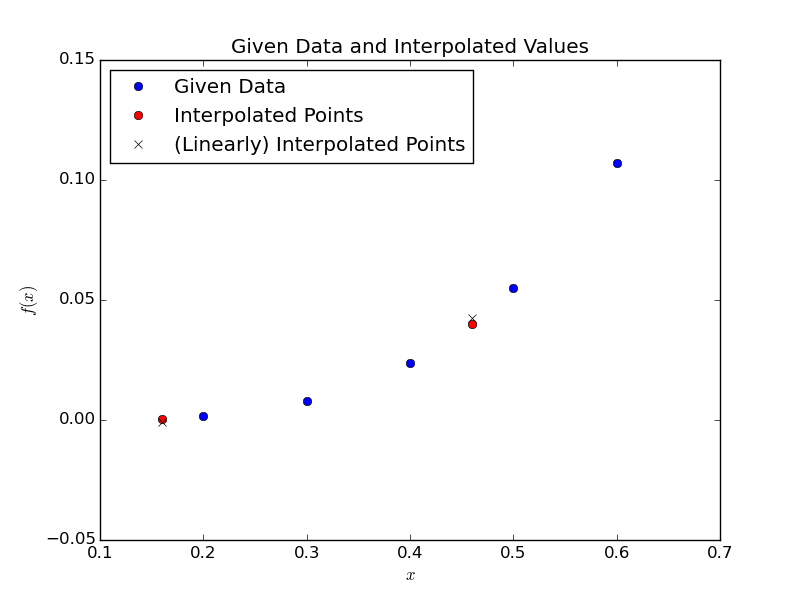
\includegraphics[width=.7\textwidth]{homework1_problem1_plot1}
  \caption{Interpolation and Extrapolation Results}
\end{figure}

The `X' points are used to compare to the interpolated values, so that both can be seen with relative ease.

The results are as follows:

\begin{verbatim}
Neville Interpolated Values:
x:  0.16  f(x):  0.00045194032  error:  0.0014827584
x:  0.46  f(x):  0.04013537472  error:  0.02792063032
Comparison to Linear:
x:  0.16  f(x):  -0.00089994  error:  0.00398499
x:  0.46  f(x):  0.042341  error:  0.057976
\end{verbatim}

\subsection{Analysis}

It was mentioned previously that a fifth power polynomial was appropriate for this problem, and that stems primarily from there being only 5 points to interpolate. Using a much higher order polynomial for a large data set, such as one with hundreds of points, is not appropriate.

\subsection{Interpretation}

The results seem very reasonable, particularly when you see them plotted. The errors for the Neville interpolation are much better than those of the linear interpolation, due to Neville's algorithm taking into account a larger amount of data. It is also of note that the extrapolated point has a much higher percent error compared to that of the interpolated point.

\subsection{Critique}

This program was designed specifically to be used for this homework problem. In particular, the interpolation returns the estimated error alongside the interpolated result. This became somewhat problematic in the second problem, where the code was copied and used, but required modification.

\subsection{Log}

The problem took approximately 7.5 hours to complete. 5 of that were writing the interpolation code, and 2 was used interpreting results, checking code on quasar, and making the code presentable. The final half-hour was used writing the calculation for section 1.3 out and making sure it looked correct.

\pagebreak

\section{Problem 2}

\subsection{Problem Statement}
Write a program to calculate the first-order and second-order derivatives of $f(x) = x^3 \cos(x)$ at
$x \in [\pi/2, \pi]$ and estimate the numerical accuracy. You may use the three-point formulas for the
calculations of the first-order and second-order derivatives. Use 100 uniform intervals in the range.
For the boundary points, you may use the formulas discussed in the class or extrapolated values by
using the linear interpolation or the Lagrange interpolation. The numerical accuracy at each x value
can be obtained by comparing with the analytical result. (15 pts)

\subsection{Method}

This program uses the three-point formulas to determine the derivative of some given function $f(x)$. Further, the second derivative is also calculated directly from $f(x)$, using a three point formula once again.

The program does not take any input, and instead generates a function based on the problem statement. In order to complete the derivative for the entire range, the endpoints on either side of the range are extrapolated using a five point, fifth-order polynomial interpolation, similar to that of Problem 1. This allows for the algorithm to be used over the entire range, without needing to worry about endpoints. From here, the derivatives are calculated using the formulas discussed in lecture.

Analytic results were found by taking the derivatives of the functions in questions, coding them in explicitly, and then evaluating them for the same set of points used to generate our $f(x)$ at the beginning. From these, the approximate errors were found, and plots of the numerical and analytic results were generated. Note that only the largest error between any one point and its analytic counterpart is shown in the results.

\subsection{Verification of Program}

As previously stated, these results were compared to the analytic results, and appear consistent.

\pagebreak

\subsection{Data}

The plot generated is included here.

\begin{figure}[h]
  \centering
    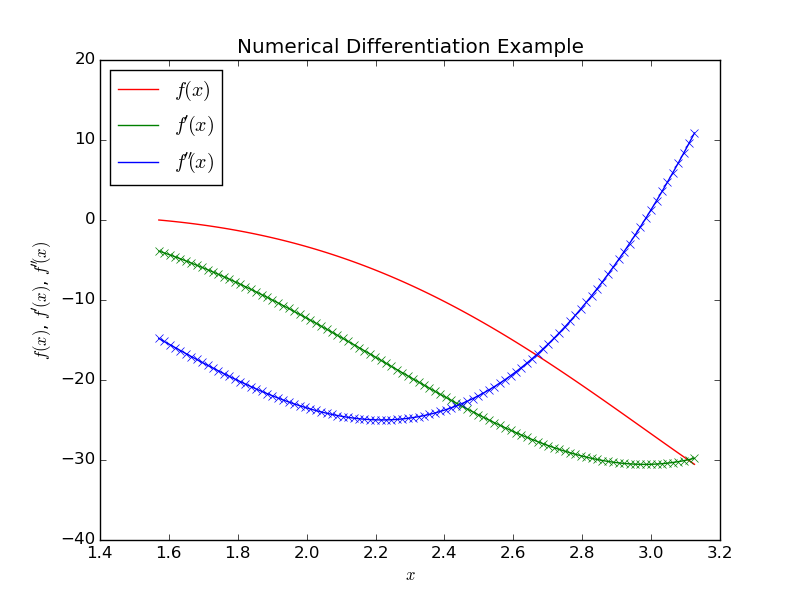
\includegraphics[width=.8\textwidth]{homework1_problem2_plot1}
  \caption{Numerical differentiation results, using a step size of $0.005\pi$.}
\end{figure}

Take note that the `X' marks have been used to show the actual (analytic) values, to be used for visual comparison. Errors have also been calculated, and the maximum and percent error shown below:

\begin{verbatim}
Max Absolute f'(x) Error:  0.00335496968799
Percent f'(x) Error:  0.0259588077833  %
Max Absolute f''(x) Error:  0.00201864228176
Percent f''(x) Error:  0.012184717569  %
\end{verbatim}

\subsection{Analysis}

In this case, we know that the target function is smooth, and should give reasonable results for the derivative. After plotting the results, it is apparent that this is the case. The results of the maximum errors are actually very accurate, which is very nice.

One issue that may arise is the use of interpolation to find the boundaries. This case happened to be a nice case, since the curve was relatively smooth at the ends. If it had a been a more oscillatory function (say, $\cos(x)$, evaluated near an extrema) the result could have a much large associated error.

\subsection{Interpretation}

The results are fairly straightforward. The derivatives are calculated directly from $f(x)$, and as such errors propagated from $f(x)$ to $f'(x)$ are not propagated to $f''(x)$.

\subsection{Critique}

This method was pretty simple, especially with the Neville's algorithm code already in place. I did need to do some modification to not return the error information, and make sure that only 5 points were used in the interpolation. Originally I had accidentally given the entire 100 point range to the interpolation code, which caused some funny, but useless results.

\subsection{Log}

This problem took approximately 4 hours. 2 hour was used to get the code in place, and 2 hours were used just correcting boundary errors.

\pagebreak

\section{Problem 3}

\subsection{Problem Statement}

Write a program to calculate the integral
$$ \int_0^1 exp(-x) dx$$
and estimate its numerical accuracy by using the Simpson rule. The numerical accuracy can be
obtained by comparing with the analytical result. (10 pts)

\subsection{Method}

This method was fairly simple. The function given in the problem statement was discretized with an even number of points explicitly. From there, the integral was found using the Simpson's Rule summation method described in class. Errors were then approximated and reported.

\subsection{Verification of Program}

This program was verified by comparing to the analytic results, which appear consistent.

\subsection{Data}

No plots were needed for these results. The results generated by the program are shown below:

\begin{verbatim}
Integral Sum:  0.624688901183
Actual Integral: 0.63212 (Approximate)
Difference:  0.00743109881669
Percent Difference:  1.17558356272 %
\end{verbatim}

\subsection{Analysis}

The approximated integral and actual result look very similar. The error looks a little large, but that's to be expected. The error scales with the $h^3$, which in this case could have been significantly smaller had more points been used.

\subsection{Interpretation}

The sum appears to be a bit of an underestimation compared to that of the analytic result. With that said, the result is still very close.

\subsection{Critique}

I had forgotten well math translates to python loops, which make this program really simple. I took more time formatting results then I did actually coding the algorithm.

One thing in particular that I tried to get a grasp on was whether Simpson's rule would consistently over or underestimate the integral, but after searching a bit it appears that Simpson's rule doesn't have a consistent behavior in this fashion.

\subsection{Log}

This code took 1 hour total to write and error correct. In total, the report document took approximately 2 hours to write.

\end{document}